%%%%%%%%%%%%%%%%%%%%%%%%%%%%%%%%%%%%%%%%%%%%%%%%%%%%%%%%%%%%%%%%%%%
%%% Documento LaTeX 																						%%%
%%%%%%%%%%%%%%%%%%%%%%%%%%%%%%%%%%%%%%%%%%%%%%%%%%%%%%%%%%%%%%%%%%%
% Título:		Capítulo 2
% Autor:  	Ignacio Moreno Doblas
% Fecha:  	2014-02-01, actualizado 2019-11-11
% Versión:	0.5.0
%%%%%%%%%%%%%%%%%%%%%%%%%%%%%%%%%%%%%%%%%%%%%%%%%%%%%%%%%%%%%%%%%%%
% !TEX root = A0.MiTFG.tex

\chapterbegin{Resultados numéricos}
\label{chp:Utiliz}
%\minitoc

\begin{sinopsis}
\label{sec:chpltx:sinop}
En este capítulo se presentan las distintas simulaciones realizadas para analizar el ensanchamiento y la distorsión de pulsos ultracortos durante su propagación en el medio atmosférico y oceánico. Las simulaciones se construyen a partir del marco teórico desarrollado en los capítulos anteriores, combinando tanto la dispersión cromática como los efectos de la turbulencia, modelada mediante los espectros de von Kármán en atmósfera y OTOPS en océano.
\end{sinopsis}

\section{Ensanchado y distorsión por dispersión cromática en propagación atmosférica}
El objetivo de este primer conjunto de simulaciones es aislar y cuantificar el efecto de la dispersión cromática en la atmósfera sobre pulsos gaussianos ultracortos. Es importante remarcar que la dispersión cromática es un fenómeno determinista, directamente provocado por la propia atmósfera como medio dispersivo. Surge de la dependencia del índice de refracción con la frecuencia, de forma que cada componente espectral del pulso viaja a distinta velocidad. Como consecuencia, incluso en ausencia de turbulencia u otros efectos aleatorios, el pulso se ensancha y distorsiona de forma predecible a lo largo de la propagación.

Las simulaciones realizadas se han implementado en Matlab a partir del script principal \texttt{propagacionPulso.m}. Este script se basa en la ecuación de Schrödinger no lineal con dispersión de segundo y tercer orden. A partir de parámetros iniciales se genera un pulso gaussiano de entrada, se calcula su evolución mediante la \acs{FFT}~(\acl{FFT}) y se compara con la solución analítica. Finalmente, se representa el pulso en transmisión y recepción en dominio temporal y frecuencial, además de imprimir parámetros relevantes. Este script principal se ayuda de funciones auxiliares para llevar a cabo toda la simulación.

\subsubsection*{Configuración base}
Esta primera simulación corresponde al caso inicial de referencia, utilizando el código base sin modificaciones. Se considera un pulso gaussiano con \textit{chirp} positivo propagándose en un canal atmosférico dispersivo. Los parámetros del pulso y del enlace se resumen en la Tabla~\ref{config_referencia_atm}.

Dado que la longitud del enlace considerada es mayor que la longitud de dispersión asociada a la dispersión de segundo orden, el pulso experimenta un ensanchamiento temporal apreciable. En este régimen, la GVD constituye el mecanismo dominante responsable de la distorsión temporal observada. Por el contrario, la contribución de la dispersión de tercer orden resulta despreciable, ya que la distancia característica a partir de la cual su efecto se vuelve relevante es muy superior a la longitud del enlace considerada.

\begin{table}[H]
\centering
\renewcommand{\arraystretch}{1.2}
\begin{tabular}{|l|c|}
\hline
\multicolumn{2}{|c|}{\textbf{Parámetros del pulso}} \\
\hline
Longitud de onda central, $\lambda_0$ & \SI{1550}{\nano\meter} \\
Anchura temporal inicial (FWHM) & \SI{0.2}{\pico\second} \\
Parámetro \textit{chirp}, $C$ & 2 \\
\hline
\multicolumn{2}{|c|}{\textbf{Parámetros del canal FSO}} \\
\hline
Distancia de propagación, $z$ & \SI{3}{\kilo\meter} \\
Altura del enlace, $h$ & \SI{500}{\meter} \\
Dispersión de segundo orden (GVD), $\beta_2$ & \SI{0.0134}{\pico\second\squared\per\kilo\meter} \\
Dispersión de tercer orden (TOD), $\beta_3$ & \SI{1.11e-5}{\pico\second\cubed\per\kilo\meter} \\
Longitud de dispersión $L_{D2}$ & \SI{1.07}{\kilo\meter} \\
Longitud de dispersión $L_{D3}$ & \SI{157}{\kilo\meter} \\
\hline
\end{tabular}
\caption{Configuración de referencia para la simulación de propagación atmosférica considerando únicamente dispersión cromática}
\label{config_referencia_atm}
\end{table}

Tras la propagación, se comparan la duración teórica del pulso obtenida mediante la solución analítica y la duración medida en la simulación. Ambos valores resultan prácticamente coincidentes, lo que confirma la consistencia del modelo. El factor de ensanchamiento, muestra que en recepción el pulso es 7.18 veces más ancho que en transmisión. Esto se confirma ya que tras la propagación obtenemos que la duración del pulso es de \SI{1.43}{\pico\second} con respecto a los \SI{0.2}{\pico\second} que duraba originalmente.

Para el resto de casos que se simularán a continuación, se parte de esta configuración de referencia y únicamente se modificarán los parámetros que se indiquen en cada caso. Respecto a las representaciones temporales, por un lado se mostrará la parte real del campo eléctrico y, por otro, el módulo de la envolvente compleja, siendo el que permite apreciar el ensanchamiento temporal.

\begin{figure}[H]
\centering
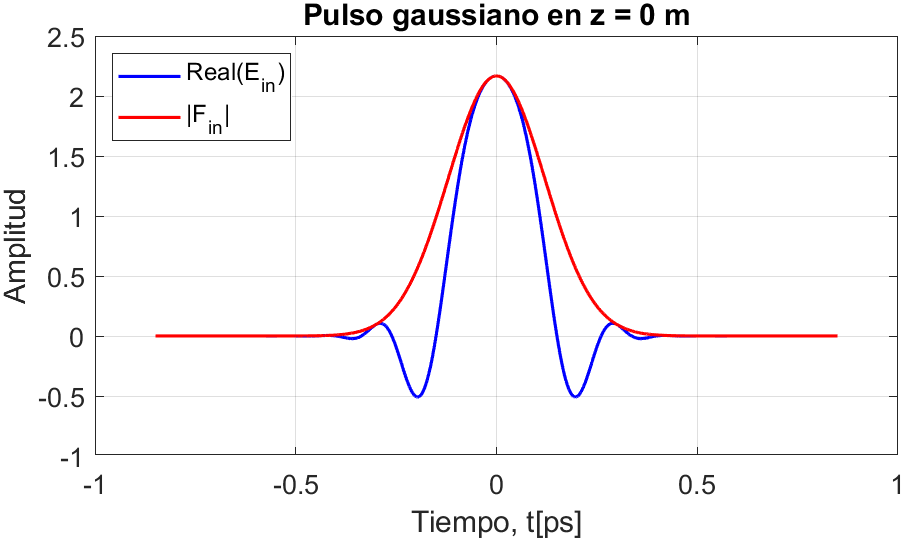
\includegraphics[width=0.8\textwidth]{figuras/Figura11.png}
\caption{Pulso gaussiano a la entrada del canal. Se representa la parte real del campo eléctrico $E_{\mathrm{in}}$ (curva azul) y el módulo de la envolvente $|F_{\mathrm{in}}|$ (curva roja)}
\label{Figura11}
\end{figure}

\begin{figure}[H]
\centering
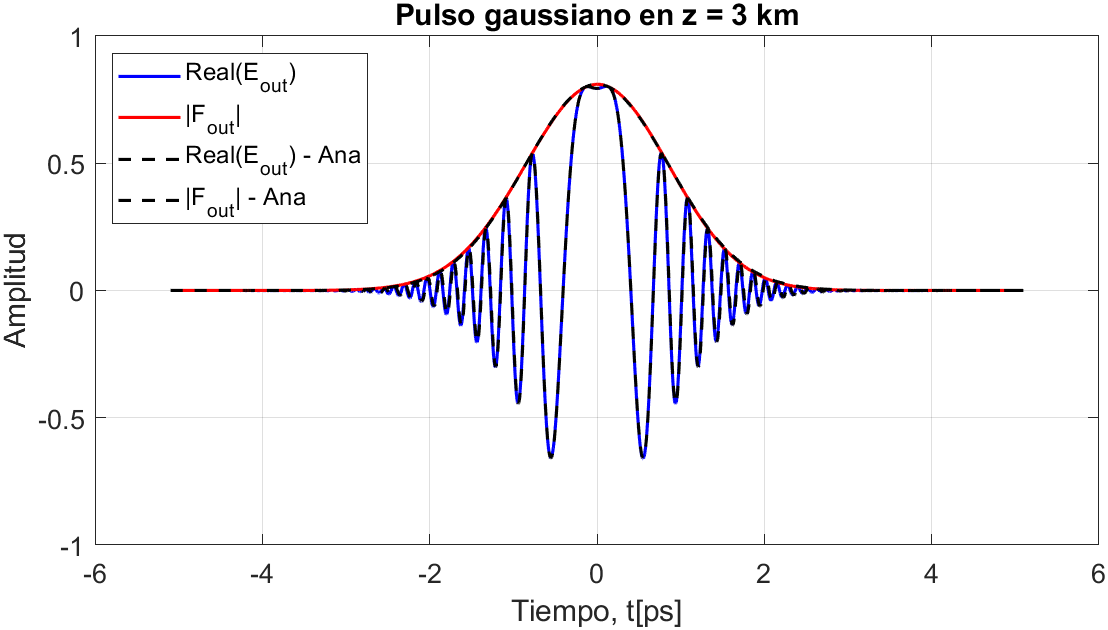
\includegraphics[width=0.8\textwidth]{figuras/Figura12.png}
\caption{Pulso gaussiano a la salida del canal. Se representa la parte real del campo eléctrico $E_{\mathrm{out}}$ (curva azul) y el módulo de la envolvente $|F_{\mathrm{out}}|$ (curva roja), junto con sus expresiones analíticas (curvas discontinuas)}
\label{Figura12}
\end{figure}

Como comprobación adicional del correcto funcionamiento del modelo numérico, se ha verificado el caso ideal en ausencia de dispersión cromática y \textit{chirp} inicial ($\beta_2=\beta_3=C=0$). En estas condiciones, la envolvente temporal del pulso se conserva invariante durante la propagación, manteniendo su anchura temporal original, tal y como se espera desde el punto de vista teórico.

\subsubsection*{Caso 2: signo en el producto $\beta_{2}C$}

En este caso se analiza la interacción entre la dispersión de segundo orden, $\beta_2$, y el \textit{chirp} inicial del pulso. Se estudian dos situaciones: cuando el producto es negativo ($\beta_{2}C < 0$) y cuando es positivo ($\beta_{2}C > 0$). Dado que en este caso únicamente se modifica el signo del \textit{chirp} inicial, las longitudes de dispersión asociadas a la dispersión de segundo y tercer orden permanecen idénticas a las del caso de referencia.

Para el caso de signo positivo se obtiene un factor de ensanchamiento de 7.18, correspondiente a una duración final del pulso de \SI{1.43}{\pico\second}. En cambio, cuando el producto es negativo, el factor de ensanchamiento es ligeramente menor, con un valor de 5.38, lo que da lugar a una duración final de \SI{1.07}{\pico\second}.

Este resultado concuerda con lo expuesto en el Capítulo 2: si $\beta_{2}C < 0$, se produce una compensación parcial del ensanchamiento debido a la interacción entre la dispersión y el \textit{chirp}. En este caso, el pulso tiende inicialmente a comprimirse hasta alcanzar una anchura mínima y, posteriormente, vuelve a ensancharse. Por el contrario, si $\beta_{2}C > 0$, ambos efectos se refuerzan, dando lugar a un ensanchamiento temporal más acusado.

Desde un punto de vista cualitativo, en el caso de signo positivo, la fase se organiza de manera que el máximo del campo coincide habitualmente con el centro del pulso, lo que se traduce en fases alineadas e interferencia constructiva. Este comportamiento está directamente determinado por la fase acumulada, gobernada por el producto $\beta_{2}C$.

\begin{figure}[H]
\centering
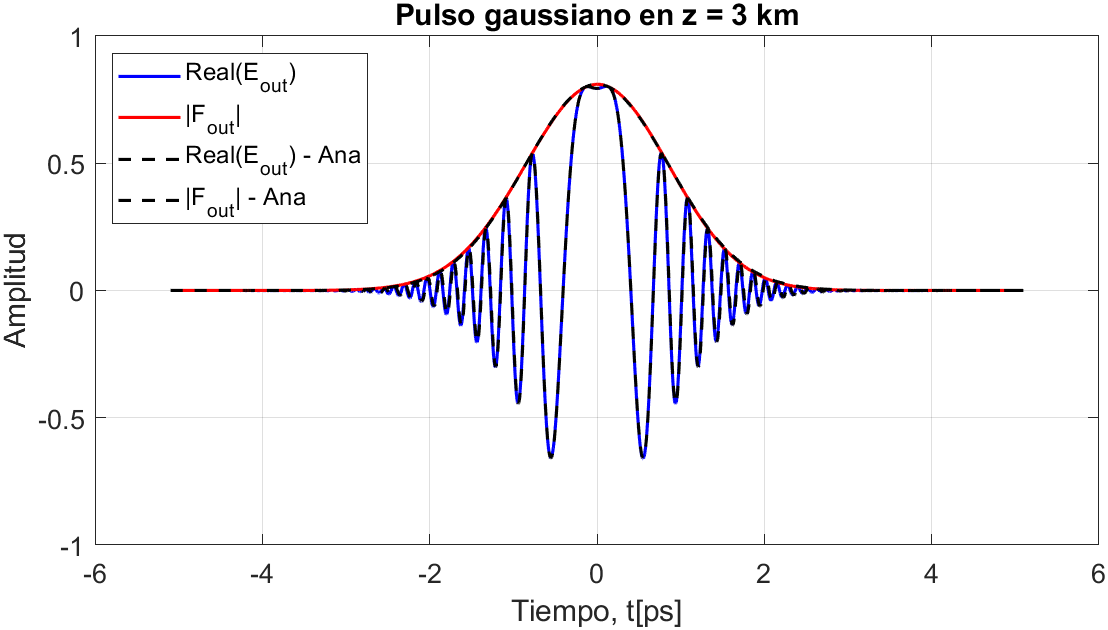
\includegraphics[width=0.8\textwidth]{figuras/Figura16.png}
\caption{Pulso gaussiano con \textit{chirp} positivo a la salida del canal, con máximo en el centro del pulso}
\label{Figura16}
\end{figure}

Para el caso de signo negativo, puede aparecer un mínimo central en el campo debido a una ligera cancelación de fases entre las componentes espectrales, asociada a fases desalineadas e interferencia parcialmente destructiva.

\begin{figure}[H]
\centering
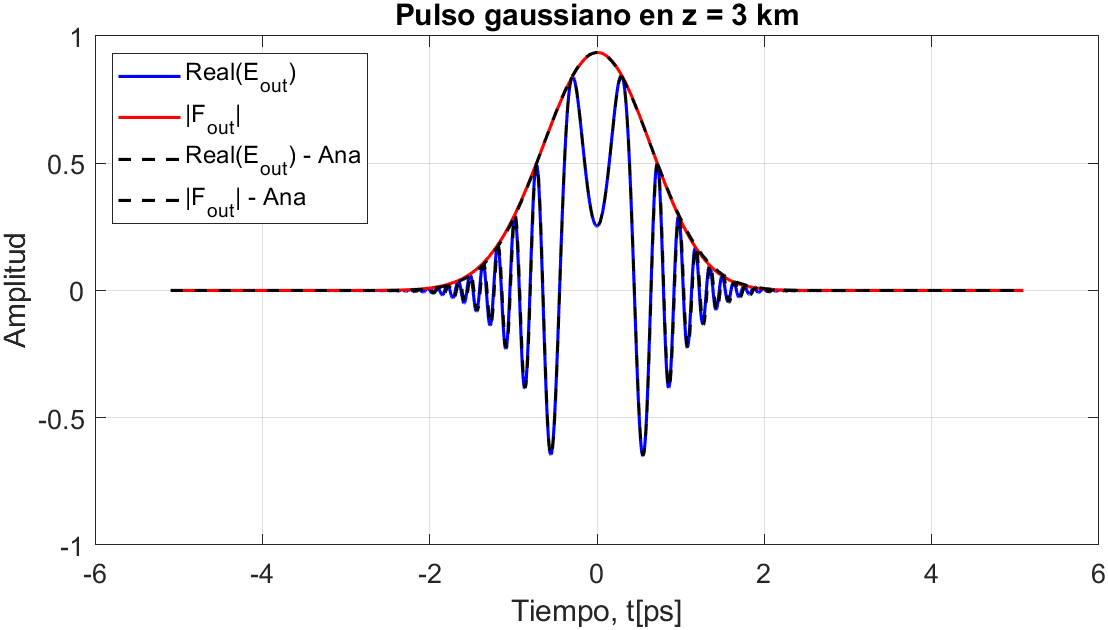
\includegraphics[width=0.8\textwidth]{figuras/Figura17.png}
\caption{Pulso gaussiano con \textit{chirp} negativo a la salida del canal, con mínimo en el centro del pulso}
\label{Figura17}
\end{figure}


\subsubsection*{Caso 3: estudio del efecto de la longitud del enlace}

En esta simulación se analiza la dependencia del ensanchamiento temporal del pulso con la distancia de propagación, manteniendo fija la configuración base. Se consideran distancias inferiores (\SI{0.5}{\kilo\metre}, \SI{1}{\kilo\metre} y \SI{2}{\kilo\metre}) y superiores (\SIrange{3}{18}{\kilo\metre}) a la distancia inicial de referencia, con el objetivo de estudiar la relación directa entre la longitud del enlace y el ensanchamiento temporal del pulso.

En la Tabla~\ref{tabla_longitud_enlace} se recogen los valores del factor de ensanchamiento y de la duración del pulso en recepción para las distintas distancias consideradas.

\begin{table}[H]
\centering
\renewcommand{\arraystretch}{1.2}
\begin{tabular}{|c|c|c|}
\hline
\textbf{Distancia [km]} & \textbf{Factor de ensanchamiento} & \textbf{Duración final [ps]} \\
\hline
0.5  & 1.98  & 0.40 \\
1    & 3.02  & 0.60 \\
2    & 5.08  & 1.01 \\
3    & 7.18  & 1.43 \\
4    & 9.24  & 1.84 \\
5    & 11.33 & 2.26 \\
10   & 21.78 & 4.35 \\
15   & 36.44 & 7.28 \\
18   & 37.44 & 7.48 \\
\hline
\end{tabular}
\caption{Evolución del ensanchamiento temporal del pulso en función de la longitud del enlace para \textit{chirp} positivo}
\label{tabla_longitud_enlace}
\end{table}

Para distancias cortas ya se observa un ensanchamiento apreciable. En particular, con tan solo \SI{0.5}{\kilo\metre} de propagación, el pulso casi duplica su duración inicial. Este resultado confirma que los efectos de dispersión cromática en pulsos ultracortos se acumulan rápidamente con la distancia, incluso antes de alcanzar la longitud de dispersión asociada a la dispersión de segundo orden. A medida que la distancia se aproxima y supera dicho umbral, el ensanchamiento se intensifica de forma notable.

Este comportamiento pone de manifiesto que, incluso en trayectos relativamente cortos, la dispersión de segundo orden combinada con \textit{chirp} positivo puede afectar de manera significativa a la forma temporal del pulso. Además, el ensanchamiento no crece de forma lineal con la distancia, sino que se acumula de manera progresivamente más acusada conforme aumenta la longitud del enlace, como consecuencia de la acumulación de fase.

\begin{figure}[H]
\centering
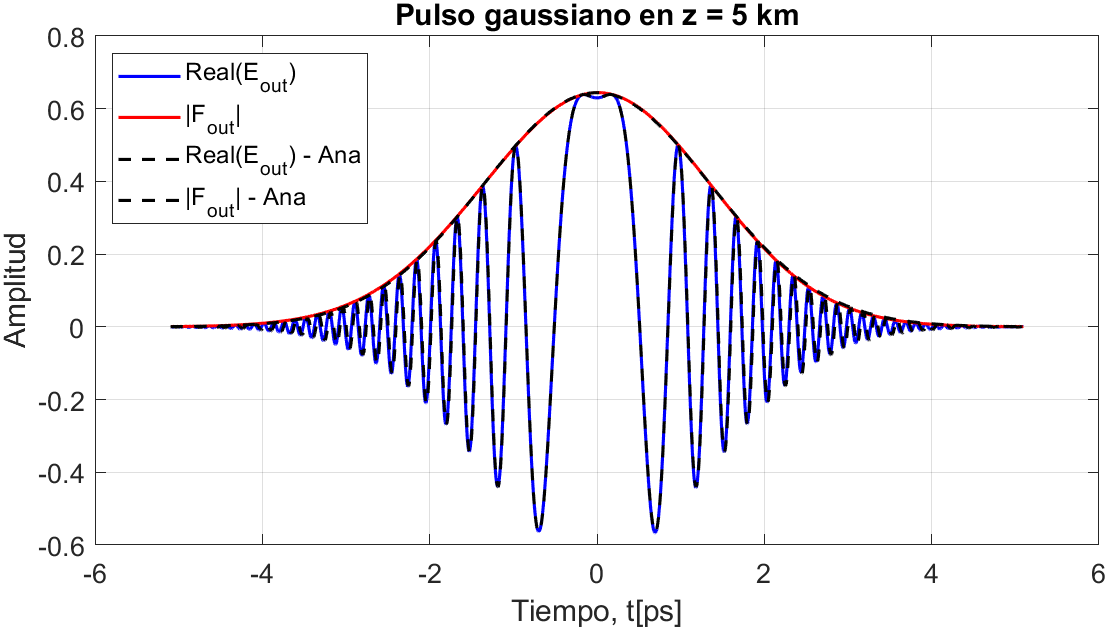
\includegraphics[width=0.8\textwidth]{figuras/Figura18.png}
\caption{Pulso gaussiano a la salida del canal tras propagarse una distancia de \SI{5}{\kilo\metre}}
\label{Figura18}
\end{figure}

\begin{figure}[H]
\centering
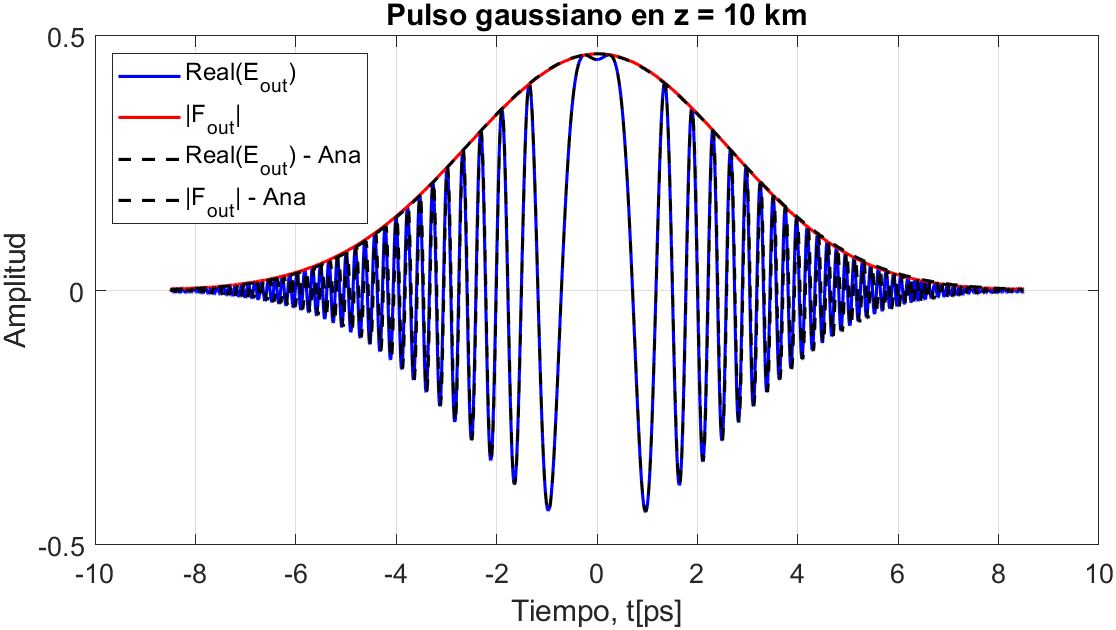
\includegraphics[width=0.8\textwidth]{figuras/Figura19.png}
\caption{Pulso gaussiano a la salida del canal tras propagarse una distancia de \SI{10}{\kilo\metre}}
\label{Figura19}
\end{figure}


\subsubsection*{Caso 4: estudio del efecto de la longitud del enlace con \textit{chirp} negativo}

En este caso se repite el mismo barrido de distancias de la simulación anterior, pero cambiando el signo del \textit{chirp} a negativo ($C=-2$), con el objetivo de analizar si la condición $\beta_2 C < 0$ actúa como un mecanismo de precompensación de la dispersión cromática y reduce el ensanchamiento temporal del pulso.

En la Tabla~\ref{tabla_longitud_enlace_chirp_negativo} se recogen los valores del factor de ensanchamiento y de la duración del pulso en recepción para las distintas distancias consideradas.

\begin{table}[H]
\centering
\renewcommand{\arraystretch}{1.2}
\begin{tabular}{|c|c|c|}
\hline
\textbf{Distancia [km]} & \textbf{Factor de ensanchamiento} & \textbf{Duración final [ps]} \\
\hline
0.5  & 0.47  & 0.09 \\
1    & 1.27  & 0.25 \\
2    & 3.32  & 0.66 \\
3    & 5.39  & 1.07 \\
4    & 7.48  & 1.49 \\
5    & 9.57  & 1.91 \\
10   & 19.85 & 3.97 \\
15   & 37.27 & 7.45 \\
18   & 16.44 & 3.28 \\
\hline
\end{tabular}
\caption{Evolución del ensanchamiento temporal del pulso en función de la longitud del enlace para \textit{chirp} negativo}
\label{tabla_longitud_enlace_chirp_negativo}
\end{table}

Para distancias cortas, se observa un comportamiento claramente distinto al caso de \textit{chirp} positivo. En particular, a \SI{0.5}{\kilo\metre} la duración del pulso en recepción se reduce hasta aproximadamente \SI{0.09}{\pico\second}, lo que confirma una compresión temporal significativa respecto a la duración original. A \SI{1}{\kilo\metre}, la duración del pulso resulta cercana a la inicial, lo que indica una compensación casi completa del ensanchamiento inducido por la dispersión cromática.

A partir de distancias del orden de \SI{2}{\kilo\metre}, la dispersión acumulada comienza a superar la capacidad del \textit{chirp} negativo para contrarrestarla y el pulso vuelve a ensancharse progresivamente, aunque con factores de ensanchamiento inferiores a los obtenidos en el caso de \textit{chirp} positivo para distancias equivalentes.

Para distancias grandes, el efecto compensador del \textit{chirp} negativo se debilita y el comportamiento del pulso tiende a asemejarse al observado con \textit{chirp} positivo.


\subsubsection*{Caso 5: cambios en la duración del pulso}

En este caso se analiza el efecto de variar la duración del pulso manteniendo constantes el resto de parámetros. Se consideran pulsos gaussianos con duraciones iniciales de \SI{0.05}{\pico\second}, \SI{0.1}{\pico\second}, \SI{0.5}{\pico\second} y \SI{1}{\pico\second}, con el objetivo de evaluar cómo la dispersión cromática se intensifica al reducir la anchura temporal del pulso.

Esta simulación permite confirmar la relación tiempo-frecuencia: cuanto más corto es un pulso en el dominio temporal, mayor es su anchura espectral y, por tanto, mayores son las diferencias de retardo de grupo entre sus componentes frecuenciales, lo que incrementa el ensanchamiento por dispersión cromática.

En la Tabla~\ref{tabla_atm_duracion_pulso} se resumen las longitudes de dispersión asociadas a la dispersión de segundo y tercer orden, el factor de ensanchamiento y la duración final del pulso en recepción para cada duración inicial considerada.


\begin{table}[H]
\centering
\hspace*{-1.4cm}
\renewcommand{\arraystretch}{1.2}
\begin{tabular}{|c|c|c|c|c|}
\hline
\textbf{FWHM inicial [ps]} & $\mathbf{L_{D2}}$ \textbf{[km]} & $\mathbf{L_{D3}}$ \textbf{[km]} & \textbf{Factor de ensanchamiento} & \textbf{Duración final [ps]} \\
\hline
0.05 & 0.06 & 2.45    & 15.64 & 0.78 \\
0.10 & 0.26 & 19.60   & 26.84 & 2.68 \\
0.50 & 6.71  & 2450.29 & 1.95  & 0.97 \\
1.00 & 26.84 & 19602.31& 1.23  & 1.23 \\
\hline
\end{tabular}
\caption{Influencia de la duración inicial del pulso en el ensanchamiento temporal tras la propagación}
\label{tabla_atm_duracion_pulso}
\end{table}

Los resultados muestran que, al reducir la duración inicial del pulso, las longitudes de dispersión disminuyen de forma significativa, situando la propagación en un régimen claramente dispersivo.

Para pulsos ultracortos de \SI{0.05}{\pico\second}, la longitud de dispersión se reduce hasta valores del orden de decenas de metros, lo que confirma la elevada sensibilidad de estos pulsos a la dispersión cromática, incluso en enlaces atmosféricos de pocos kilómetros.

Por el contrario, al aumentar la duración del pulso hasta \SI{0.5}{\pico\second} y \SI{1}{\pico\second}, las longitudes de dispersión crecen notablemente y el ensanchamiento se atenúa de forma clara, obteniéndose factores cercanos a la unidad. 

Estos resultados ponen de manifiesto que, aunque los pulsos ultracortos permiten mayores tasas de transmisión, su mayor sensibilidad a la dispersión exige técnicas de compensación dispersiva para preservar la integridad temporal del pulso en distancias de interés.

\begin{figure}[H]
\centering
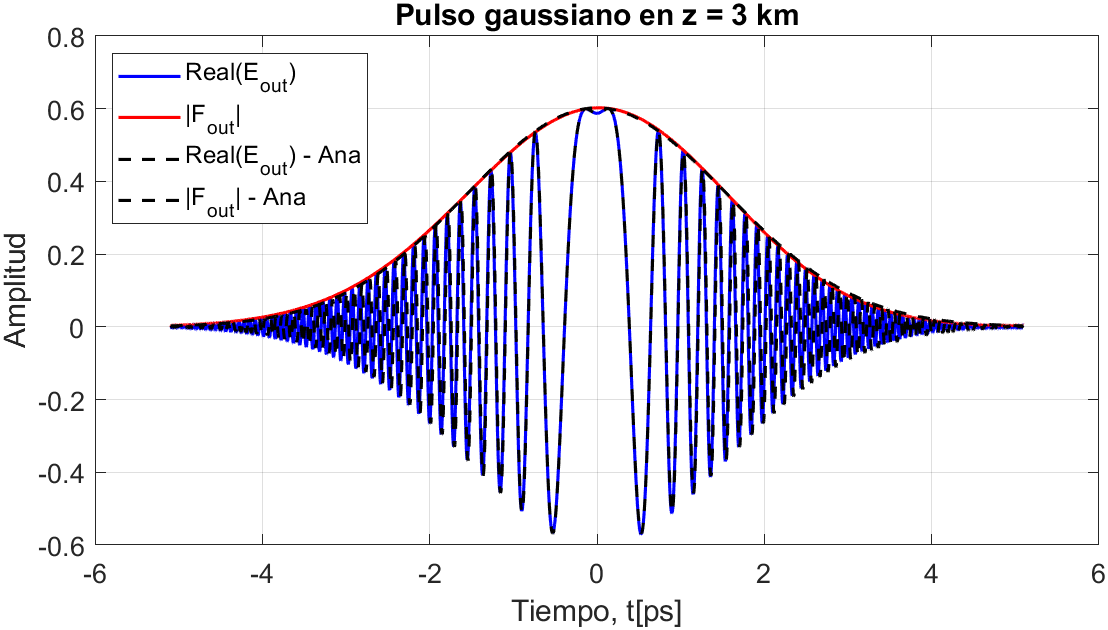
\includegraphics[width=0.9\textwidth]{figuras/Figura21.png}
\caption{Pulso gaussiano a la salida del canal con duración inicial de \SI{0.1}{\pico\second}}
\label{Figura21}
\end{figure}



\section{Ensanchado y distorsión por dispersión cromática en propagación oceánica}

Tras el análisis en el canal atmosférico, este segundo bloque de simulaciones se centra en el medio oceánico. El objetivo fundamental es realizar una evaluación comparativa del impacto de la dispersión cromática en el medio oceánico frente al atmosférico. 

Para modelar este comportamiento con precisión, se ha tomado como base el script elaborado para la atmósfera, adaptándolo a las particularidades del océano e introduciendo cambios necesarios en las siguientes funciones auxiliares:


\begin{itemize}
    \item \textbf{Modelado del medio (\texttt{canalOcean.m}):} Se ha implementado un cálculo preciso de los parámetros de dispersión basado en el modelo del índice de refracción del agua de mar. En esta función auxiliar, se han ajustado las fórmulas de las longitudes de dispersión ($L_{D2}$ y $L_{D3}$) para ser totalmente coherentes con la formulación teórica basada en la FWHM y el factor $\ln(2)$:
    \[ L_{D2} = \frac{FWHM^2}{4 \ln(2) |\beta_2|}, \quad L_{D3} = \frac{FWHM^3}{8 (\ln(2))^2 |\beta_3|} .\]

    \item \textbf{Configuración de la malla temporal:} Dada la disparidad de escalas entre el pulso inicial y el pulso tras propagarse por el océano (cientos de ps), se ha modificado el script principal para implementar una malla temporal de alta resolución mediante la función auxiliar \texttt{auto\_time\_grid\_m}. Se ha configurado una densidad de hasta $2^{19}$ puntos de muestreo, lo que permite capturar simultáneamente el pulso en transmisión y recepción sin perder precisión numérica ni sufrir efectos de \textit{aliasing}.
\end{itemize}

\subsubsection*{Configuración base}

Esta simulación constituye el caso de referencia para el medio acuático, utilizando el código adaptado específicamente para las propiedades ópticas del agua de mar. Los parámetros del pulso y del canal oceánico se detallan en la 
Tabla~\ref{config_referencia_oceano}.

En este escenario, se observa que la longitud del enlace es cientos de veces superior a la longitud de dispersión de segundo orden, lo que sitúa la propagación en un régimen de dispersión extrema. A pesar de que la distancia es corta en comparación con los kilómetros utilizados en la atmósfera, el ensanchamiento temporal es órdenes de magnitud superior debido a que el coeficiente $\beta_2$ en el agua es mucho más elevado. Asimismo, aunque el efecto de la GVD es el predominante, la longitud de dispersión de tercer orden es ahora comparable a la distancia del enlace, lo que justifica la inclusión de $\beta_3$ para garantizar la precisión del modelo. 

\begin{table}[H]
\centering
\renewcommand{\arraystretch}{1.2}
\begin{tabular}{|l|c|}
\hline
\multicolumn{2}{|c|}{\textbf{Parámetros del pulso}} \\
\hline
Longitud de onda central, $\lambda_0$ & \SI{500}{\nano\meter} \\
Anchura temporal inicial (FWHM) & \SI{0.2}{\pico\second} \\
Parámetro \textit{chirp}, $C$ & 2 \\
\hline
\multicolumn{2}{|c|}{\textbf{Parámetros del canal oceánico}} \\
\hline
Distancia de propagación, $z$ & \SI{100}{\meter} \\
Dispersión de segundo orden (GVD), $\beta_2$ & \SI{0.0626}{\pico\second\squared\per\meter} \\
Dispersión de tercer orden (TOD), $\beta_3$ & \SI{2.6942e-5}{\pico\second\cubed\per\meter} \\
Longitud de dispersión $L_{D2}$ & \SI{0.23}{\meter} \\
Longitud de dispersión $L_{D3}$ & \SI{77.25}{\meter} \\
\hline
\end{tabular}
\caption{Configuración de referencia para la simulación de propagación en océano considerando únicamente dispersión cromática}
\label{config_referencia_oceano}
\end{table}

Tras la propagación, se comparan los resultados de la simulación numérica frente a la solución analítica. Se observa una concordancia casi total, validando la robustez de la malla temporal adaptativa empleada. El factor de ensanchamiento resultante es extraordinariamente alto, situándose en 971.15. Esto implica que el pulso pasa de una duración inicial de \SI{0.2}{\pico\second} a una duración en recepción de aproximadamente \SI{194.31}{\pico\second}.

\begin{figure}[H]
\centering
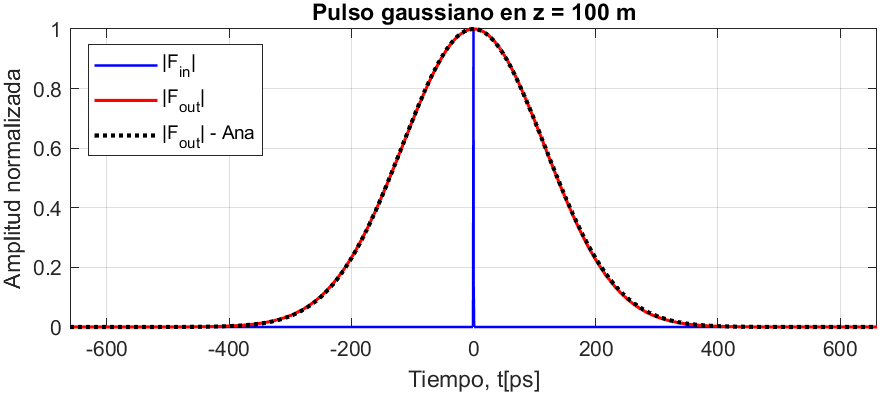
\includegraphics[width=1\textwidth]{figuras/Figura37.png}
\caption{Comparación temporal del módulo normalizado de la envolvente del pulso gaussiano. Se muestran la señal a la entrada (curva azul), la salida simulada (curva roja) y la solución analítica (curva negra)}
\label{fig_oceano_base}
\end{figure}

Como se aprecia en la Figura~\ref{fig_oceano_base}, la envolvente temporal en recepción se ensancha masivamente, ocupando una ventana temporal de varios cientos de picosegundos. A diferencia de las gráficas obtenidas en el canal atmosférico, aquí se representa la intensidad normalizada. Debido al factor de ensanchamiento extremo, la visualización de las oscilaciones de la portadora resultaría impracticable en esta escala temporal, por lo que la comparativa visual se centra en la expansión de la envolvente.

\subsubsection*{Caso 2: signo en el producto $\beta_{2}C$}

En este caso se analiza la influencia del signo del producto $\beta_{2}C$ en la propagación del pulso gaussiano a través del canal oceánico. Al igual que en el caso atmosférico, se consideran dos situaciones: cuando el producto es positivo ($\beta_{2}C > 0$) y cuando es negativo ($\beta_{2}C < 0$).

Los resultados obtenidos muestran que, a diferencia del caso atmosférico, el signo del producto $\beta_{2}C$ apenas introduce diferencias apreciables en el ensanchamiento temporal del pulso en el medio oceánico. Para ambos signos, la anchura temporal a la salida del canal es prácticamente la misma, con valores cercanos a \SI{194}{\pico\second}. De forma más precisa, se obtienen duraciones finales de \SI{194.31}{\pico\second} para signo positivo y de \SI{193.95}{\pico\second} para signo negativo, con factores de ensanchamiento de 971.59 y 969.80, respectivamente, lo que confirma que las diferencias entre ambos casos son despreciables.

Este comportamiento se debe a la fuerte dispersión cromática del medio oceánico. En este régimen, el ensanchamiento del pulso está dominado por la dispersión de segundo orden, lo que hace que el efecto compensador o reforzador del \textit{chirp} inicial sea prácticamente nulo.

Además, no se observan diferencias significativas en la forma del pulso entre ambos casos.
 

\subsubsection*{Caso 3: estudio del efecto de la longitud del enlace}

En esta simulación se analiza la dependencia del ensanchamiento temporal del pulso con la distancia de propagación en el medio oceánico, manteniendo fija la configuración base. A diferencia del caso atmosférico, las distancias consideradas son del orden de decenas de metros debido a los elevados valores de dispersión característicos del agua.

Se estudian distintas longitudes de enlace: \SI{10}{\meter}, \SI{25}{\meter}, \SI{50}{\meter}, \SI{75}{\meter} y \SI{100}{\meter}, todas ellas muy superiores a la longitud de dispersión asociada a la dispersión de segundo orden.

En la Tabla~\ref{tabla_oceano_distancia_disp} se recogen los valores del factor de ensanchamiento y de la duración del pulso en recepción para las distintas distancias consideradas.

\begin{table}[H]
\centering
\renewcommand{\arraystretch}{1.2}
\begin{tabular}{|c|c|c|}
\hline
\textbf{Distancia [m]} & \textbf{Factor de ensanchamiento} & \textbf{Duración final [ps]} \\
\hline
10  & 97.96  & 19.59 \\
25  & 243.57 & 48.71 \\
50  & 486.24 & 97.25 \\
75  & 728.92 & 145.78 \\
100 & 971.59 & 194.32 \\
\hline
\end{tabular}
\caption{ Evolución del ensanchamiento temporal del pulso en función de la longitud del enlace
para \textit{chirp} positivo}
\label{tabla_oceano_distancia_disp}
\end{table}

Los resultados muestran que el pulso entra en un régimen fuertemente dispersivo desde distancias muy cortas. En particular, para una longitud de enlace de tan solo \SI{10}{\meter}, el factor de ensanchamiento alcanza ya un valor cercano a 98.

A medida que la distancia de propagación aumenta, el ensanchamiento crece de forma extremadamente acusada. Para distancias de \SI{25}{\meter} y \SI{50}{\meter}, el pulso alcanza duraciones del orden de varias decenas de picosegundos, mientras que a \SI{100}{\meter} la duración del pulso en recepción supera los \SI{190}{\pico\second}, lo que supone un ensanchamiento cercano a tres órdenes de magnitud respecto a la duración inicial.

Este comportamiento contrasta fuertemente con el observado en el medio atmosférico, donde el ensanchamiento se desarrolla de forma progresiva a lo largo de kilómetros. En el medio oceánico, la elevada magnitud del parámetro de dispersión de segundo orden provoca una acumulación muy rápida de fase dispersiva, lo que limita severamente la transmisión de pulsos ultracortos incluso para distancias de propagación relativamente reducidas. Por este motivo, no se contemplan distancias de propagación mayores en este estudio, ya que los elevados factores de ensanchamiento obtenidos hacen que la transmisión de pulsos ultracortos resulte impracticable en escenarios reales con la tecnología disponible actualmente.


\subsubsection*{Caso 4: estudio del efecto de la longitud del enlace con \textit{chirp} negativo}

En este caso se repite el estudio de la dependencia del ensanchamiento temporal del pulso con la distancia de propagación en el medio oceánico, manteniendo la misma configuración base pero cambiando el signo del \textit{chirp} a negativo. El objetivo es analizar de nuevo si la condición $\beta_2 C < 0$ introduce algún efecto de compensación apreciable.

Se consideran las mismas longitudes de enlace que en el caso de \textit{chirp} positivo.

En la Tabla~\ref{tabla_oceano_distancia_disp_chirp_neg} se recogen los valores del factor de ensanchamiento y de la duración del pulso en recepción para las distintas distancias consideradas.

\begin{table}[H]
\centering
\renewcommand{\arraystretch}{1.2}
\begin{tabular}{|c|c|c|}
\hline
\textbf{Distancia [m]} & \textbf{Factor de ensanchamiento} & \textbf{Duración final [ps]} \\
\hline
10  & 96.18  & 19.24 \\
25  & 241.78 & 48.36 \\
50  & 484.45 & 96.89 \\
75  & 727.13 & 145.43 \\
100 & 969.80 & 193.96 \\
\hline
\end{tabular}
\caption{Evolución del ensanchamiento temporal del pulso en función de la longitud del enlace para \textit{chirp} negativo}
\label{tabla_oceano_distancia_disp_chirp_neg}
\end{table}

Los resultados obtenidos muestran que, al igual que en el caso de \textit{chirp} positivo, el pulso entra en un régimen fuertemente dispersivo desde distancias muy cortas.

\subsubsection*{Caso 5: cambios en la duración del pulso}

En este caso se estudia el efecto de variar la duración temporal del pulso manteniendo constantes los restantes parámetros. Se analizan de nuevo pulsos gaussianos con duraciones iniciales de \SI{0.05}{\pico\second}, \SI{0.1}{\pico\second}, \SI{0.5}{\pico\second} y \SI{1}{\pico\second}


En la Tabla~\ref{tabla_oceano_duracion_pulso} se resumen las longitudes de dispersión asociadas a la dispersión de segundo y tercer orden, el factor de ensanchamiento y la duración final del pulso en recepción para cada duración inicial considerada.


\begin{table}[H]
\centering
\hspace*{-1.2cm}
\renewcommand{\arraystretch}{1.2}
\begin{tabular}{|c|c|c|c|c|}
\hline
\textbf{FWHM inicial [ps]} & $\mathbf{L_{D2}}$ \textbf{[m]} & $\mathbf{L_{D3}}$ \textbf{[m]} & \textbf{Factor de ensanchamiento} & \textbf{Duración final [ps]} \\
\hline
0.05 & 0.014 & 1.21  & 15533.88 & 776.69 \\
0.10 & 0.058 & 9.66  & 3883.77  & 388.38 \\
0.50 & 1.44  & 1207  & 156.21   & 78.10  \\
1.00 & 5.76  & 9657  & 39.72    & 39.72  \\
\hline
\end{tabular}
\caption{Influencia de la duración inicial del pulso en el ensanchamiento temporal tras la propagación}
\label{tabla_oceano_duracion_pulso}
\end{table}


Los resultados muestran que la reducción de la duración inicial del pulso tiene un impacto extremadamente severo en el ensanchamiento temporal en el medio oceánico. Para pulsos ultracortos, las longitudes de dispersión de segundo orden son del orden de centímetros. Como consecuencia, se alcanzan factores de ensanchamiento superiores a $10^3$, dando lugar a duraciones finales del orden de cientos de picosegundos.

Al aumentar la duración inicial del pulso, las longitudes de dispersión crecen y el ensanchamiento se atenúa progresivamente.

Estos resultados confirman que, en el medio oceánico, la reducción de la duración del pulso tiene un efecto mucho más crítico que en el caso atmosférico. Los pulsos se degradan de forma extrema debido a la elevada dispersión cromática y esto limita severamente su viabilidad práctica.

\section{Ensanchado y distorsión por dispersión cromática y turbulencia en propagación atmosférica}
En este siguiente bloque de simulaciones, se analiza la propagación de pulsos ultracortos a través de un enlace atmosférico considerando de forma conjunta los efectos de la dispersión cromática y la turbulencia del medio. Para ello, se emplea el script \texttt{propagacionPulso\_turb.m}, que extiende el modelo de propagación puramente dispersivo incorporando la influencia de la turbulencia atmosférica mediante funciones espectrales basadas en el modelo de von Kármán.

El ensanchamiento temporal del pulso se cuantifica mediante el factor de ensanchamiento \acs{BF}~(\acl{BF}), definido como la relación entre la anchura temporal del pulso a la salida del enlace y su anchura inicial. La duración final del pulso en términos de FWHM se obtiene directamente como:

\begin{equation}
\mathrm{FWHM}_{\mathrm{out}} = BF \cdot \mathrm{FWHM}_{\mathrm{in}}.
\end{equation}

En el escenario atmosférico, el cálculo del factor de ensanchamiento se realiza siguiendo la formulación implementada en una de las funciones incluidas en el conjunto de códigos de partida proporcionados, utilizada como base para el desarrollo de las simulaciones y que extiende el modelo puramente dispersivo incorporando los efectos de la turbulencia atmosférica mediante el espectro de von Kármán.

El efecto de la turbulencia atmosférica se modela a partir de dicho espectro, obteniéndose un término de ensanchamiento temporal \acs{TPS}~(\acl{TPS}) que depende del parámetro $C_n^2$, de la distancia de propagación y de la escala externa de turbulencia. A partir de este término, el factor de ensanchamiento asociado exclusivamente a la turbulencia se calcula como: 

\begin{equation}
BF_{\mathrm{turb}} = \sqrt{1 + TPS}.
\end{equation}

Por su parte, el ensanchamiento introducido por la dispersión cromática se evalúa mediante una expresión general para pulsos gaussianos que incluye la presencia de \textit{chirp} inicial, así como los efectos de la dispersión de segundo y tercer orden. Esta formulación, implementada en la función \texttt{factorEnsanchado.m}, permite analizar escenarios más generales que los descritos por expresiones analíticas simplificadas.


El efecto conjunto de la dispersión cromática y la turbulencia se obtiene combinando ambas contribuciones a nivel de varianza temporal, siguiendo la estructura de cálculo empleada en el código de referencia.

Cabe destacar que, frente a expresiones analíticas disponibles en la literatura válidas únicamente para pulsos sin \textit{chirp} y considerando únicamente dispersión de segundo orden, el modelo empleado en este trabajo permite incorporar \textit{chirp} inicial y términos de dispersión de orden superior, lo que justifica su utilización para el análisis de pulsos ultracortos en escenarios atmosféricos realistas.

En todos los casos analizados a lo largo de este bloque, las simulaciones se realizan para pulsos y parámetros del enlace concretos, fijando la duración inicial del pulso, la distancia de propagación y el régimen de turbulencia, entre otros.

No obstante, en el caso de configuración base se incluye adicionalmente un barrido del factor de ensanchamiento temporal en función de la anchura eficaz del pulso. El objetivo de estas representaciones es proporcionar una visión global del comportamiento del sistema bajo cada régimen de turbulencia. Este barrido permite identificar de forma clara qué mecanismo domina el ensanchamiento temporal en cada situación. 

\subsubsection*{Configuración base}
En este caso se analiza la propagación de un pulso gaussiano a través de un enlace atmosférico considerando simultáneamente los efectos de la dispersión cromática y la turbulencia atmosférica. Se parte de la configuración base utilizada en el estudio con dispersión únicamente.

Con el fin de evaluar la influencia de la intensidad de la turbulencia, se consideran tres regímenes distintos: turbulencia débil, turbulencia moderada y turbulencia fuerte, caracterizados por diferentes valores del parámetro $C_n^2$.

\paragraph{Régimen de turbulencia débil}\\
En primer lugar se analiza el caso de turbulencia débil, correspondiente a $C_n^2 = 10^{-17}\,\mathrm{m^{-2/3}}$. En la Tabla~\ref{tabla_atm_comb_debil} se resumen los factores de ensanchamiento asociados a la dispersión, a la turbulencia y al efecto combinado, así como la duración final del pulso en recepción.


\begin{table}[H]
\centering
\hspace*{-0.6cm}
\renewcommand{\arraystretch}{1.2}
\begin{tabular}{|l|c|}
\hline
\multicolumn{2}{|c|}{\textbf{Turbulencia débil}}\\
\hline
Factor de ensanchamiento por dispersión, $BF_{\mathrm{disp}}$ & 7.15 \\
Factor de ensanchamiento por turbulencia, $BF_{\mathrm{turb}}$ & 1.00 \\
Factor de ensanchamiento total, $BF_{\mathrm{total}}$ & 7.15 \\
\hline
Duración final por dispersión [ps] & 1.43 \\
Duración final por turbulencia [ps] & 0.20 \\
Duración final total [ps] & 1.43 \\
\hline
\end{tabular}
\caption{Resultados del efecto combinado de dispersión cromática y turbulencia débil en un enlace atmosférico}
\label{tabla_atm_comb_debil}
\end{table}

En este régimen, el factor de ensanchamiento asociado a la turbulencia es prácticamente unitario, por lo que el comportamiento del pulso está dominado por la dispersión cromática. La duración final del pulso coincide prácticamente con la obtenida en el caso sin turbulencia, lo que indica que los efectos turbulentos son despreciables bajo estas condiciones.


\begin{figure}[H]
\centering
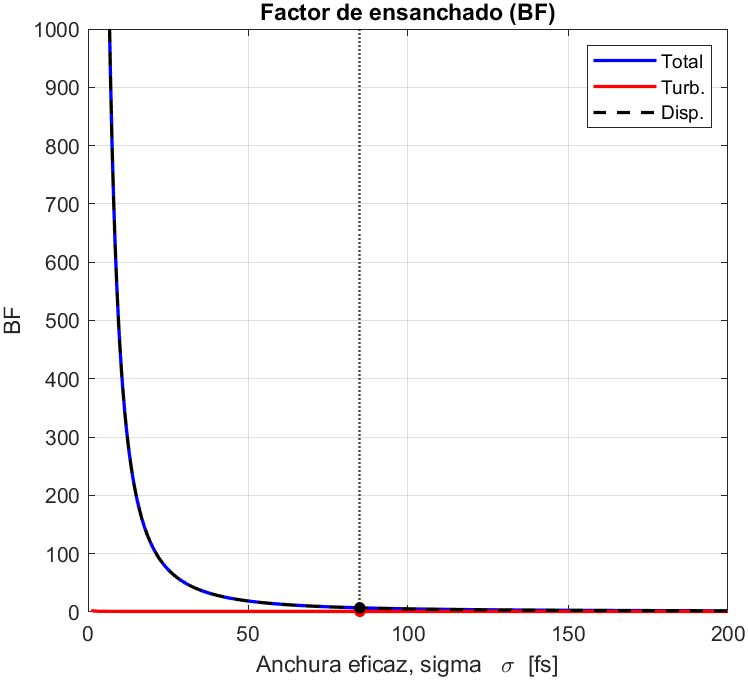
\includegraphics[width=0.9\textwidth]{figuras/atm_comb_C1_17.png}
\caption{Barrido del factor de ensanchado en función de la anchura eficaz del pulso para un enlace atmosférico, considerando dispersión cromática y turbulencia débil}
\label{fig_comb_debil}
\end{figure}

\paragraph{Régimen de turbulencia moderada}\\
A continuación, se considera un régimen de turbulencia moderada, caracterizado por un valor de $C_n^2 = 10^{-13}\,\mathrm{m^{-2/3}}$. Los resultados obtenidos se recogen en la Tabla~\ref{tabla_atm_comb_moderada}.


\begin{table}[H]
\centering
\hspace*{-0.6cm}
\renewcommand{\arraystretch}{1.2}
\begin{tabular}{|l|c|}
\hline
\multicolumn{2}{|c|}{\textbf{Turbulencia moderada}}\\
\hline
Factor de ensanchamiento por dispersión, $BF_{\mathrm{disp}}$ & 7.15 \\
Factor de ensanchamiento por turbulencia, $BF_{\mathrm{turb}}$ & 3.23 \\
Factor de ensanchamiento total, $BF_{\mathrm{total}}$ & 7.79 \\
\hline
Duración final por dispersión [ps] & 1.43 \\
Duración final por turbulencia [ps] & 0.64 \\
Duración final total [ps] & 1.55 \\
\hline
\end{tabular}
\caption{Resultados del efecto combinado de dispersión cromática y turbulencia moderada en un enlace atmosférico}
\label{tabla_atm_comb_moderada}
\end{table}

En este caso, la turbulencia introduce un ensanchamiento adicional apreciable, incrementando el factor de ensanchamiento total respecto al caso puramente dispersivo, no obstante, la dispersión cromática continúa teniendo un peso significativo en la evolución temporal del pulso.


\begin{figure}[H]
\centering
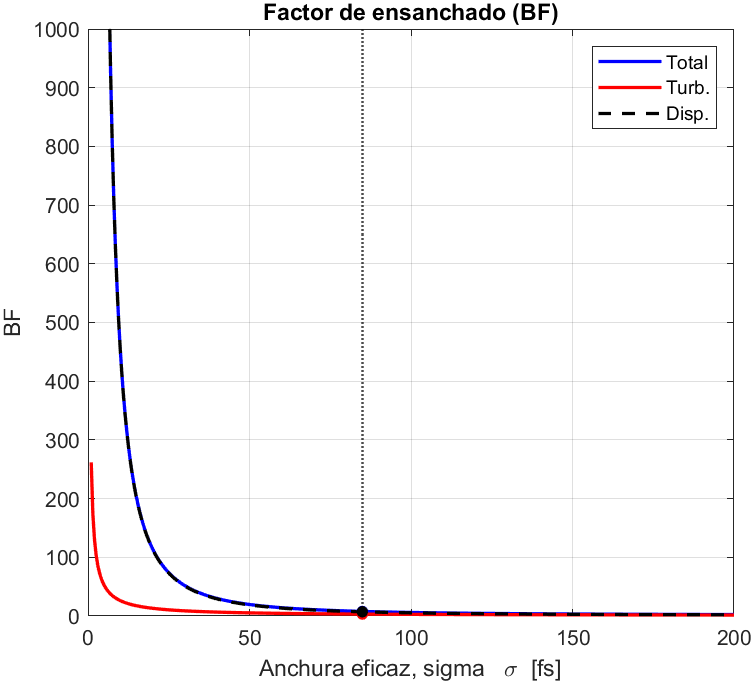
\includegraphics[width=0.9\textwidth]{figuras/atm_comb_C1_13.png}
\caption{Barrido del factor de ensanchado en función de la anchura eficaz del pulso para un enlace atmosférico, considerando dispersión cromática y turbulencia moderada}
\label{fig_comb_moderada}
\end{figure}

\paragraph{Régimen de turbulencia fuerte}\\
Finalmente, se analiza el caso de turbulencia fuerte, caracterizado por un valor elevado de $C_n^2 = 10^{-12}\,\mathrm{m^{-2/3}}$. En este régimen, los efectos turbulentos se vuelven dominantes y tienen una influencia decisiva en la evolución temporal del pulso, superando al ensanchamiento introducido por la dispersión cromática.


\begin{table}[H]
\centering
\hspace*{-0.6cm}
\renewcommand{\arraystretch}{1.2}
\begin{tabular}{|l|c|}
\hline
\multicolumn{2}{|c|}{\textbf{Turbulencia fuerte}}\\
\hline
Factor de ensanchamiento por dispersión, $BF_{\mathrm{disp}}$ & 7.15 \\
Factor de ensanchamiento por turbulencia, $BF_{\mathrm{turb}}$ & 9.79 \\
Factor de ensanchamiento total, $BF_{\mathrm{total}}$ & 12.09 \\
\hline
Duración final por dispersión [ps] & 1.43 \\
Duración final por turbulencia [ps] & 1.95 \\
Duración final total [ps] & 2.41 \\
\hline
\end{tabular}
\caption{Resultados del efecto combinado de dispersión cromática y turbulencia fuerte en un enlace atmosférico}
\label{tabla_atm_comb_fuerte}
\end{table}


\begin{figure}[H]
\centering
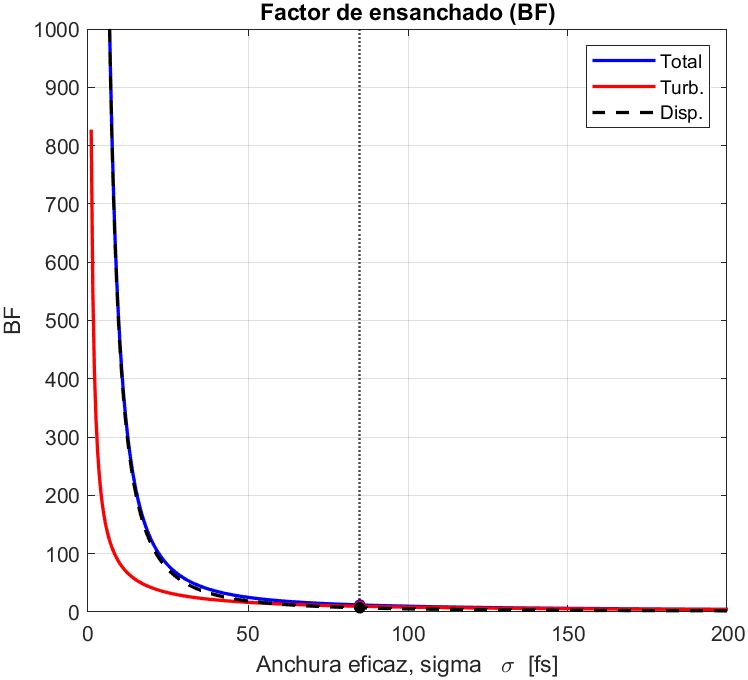
\includegraphics[width=0.9\textwidth]{figuras/atm_comb_C1_12.png}
\caption{Barrido del factor de ensanchado en función de la anchura eficaz del pulso para un enlace atmosférico, considerando dispersión cromática y turbulencia fuerte}
\label{fig_comb_fuerte}
\end{figure}



\subsubsection*{Caso 2: signo en el producto $\beta_{2}C$}
En este caso se analiza la influencia del signo del producto $\beta_{2}C$ cuando se consideran simultáneamente la dispersión cromática y la turbulencia atmosférica. Se mantiene la configuración base y se evalúa el comportamiento para tres regímenes turbulentos.


\paragraph{Régimen de turbulencia débil}\\
Para turbulencia débil, el efecto turbulento es prácticamente despreciable por lo que el ensanchamiento queda dominado por la dispersión cromática. En esta situación, el signo negativo del producto $\beta_{2}C$ reduce el ensanchamiento respecto al caso con signo positivo, actuando como una compensación parcial del efecto dispersivo.

\begin{table}[H]
\centering
\hspace*{-0.6cm}
\renewcommand{\arraystretch}{1.2}
\begin{tabular}{|l|c|}
\hline
\multicolumn{2}{|c|}{\textbf{Turbulencia débil}} \\
\hline
Factor de ensanchamiento por dispersión, $BF_{\mathrm{disp}}$ & 5.37 \\
Factor de ensanchamiento por turbulencia, $BF_{\mathrm{turb}}$ & 1.00 \\
Factor de ensanchamiento total, $BF_{\mathrm{total}}$ & 5.37 \\
\hline
Duración final por dispersión [ps] & 1.07 \\
Duración final por turbulencia [ps] & 0.20 \\
Duración final total [ps] & 1.07 \\
\hline
\end{tabular}
\caption{Resultados para signo negativo en el producto $\beta_2 C < 0$ en régimen de turbulencia débil}
\label{tabla_atm_signo_debil_Cneg}
\end{table}



\paragraph{Régimen de turbulencia moderada}\\
En turbulencia moderada, la turbulencia introduce un ensanchamiento adicional apreciable. Sin embargo, el signo negativo del producto $\beta_2C$ sigue reduciendo el término dispersivo respecto al caso con signo positivo, y el ensanchamiento total resultante es inferior.


\begin{table}[H]
\centering
\hspace*{-0.6cm}
\renewcommand{\arraystretch}{1.2}
\begin{tabular}{|l|c|}
\hline
\multicolumn{2}{|c|}{\textbf{Turbulencia moderada}} \\
\hline
Factor de ensanchamiento por dispersión, $BF_{\mathrm{disp}}$ & 5.37 \\
Factor de ensanchamiento por turbulencia, $BF_{\mathrm{turb}}$ & 3.23 \\
Factor de ensanchamiento total, $BF_{\mathrm{total}}$ & 6.19 \\
\hline
Duración final por dispersión [ps] & 1.07 \\
Duración final por turbulencia [ps] & 0.64 \\
Duración final total [ps] & 1.23 \\
\hline
\end{tabular}
\caption{Resultados para signo negativo en el producto $\beta_2 C < 0$ en régimen de turbulencia moderada}
\label{tabla_atm_signo_moderada_Cneg}
\end{table}


\paragraph{Régimen de turbulencia fuerte}\\
Finalmente, en turbulencia fuerte, el ensanchamiento está dominado por la turbulencia. En este régimen, aunque el signo negativo del producto $\beta_2C$ sigue reduciendo el ensanchamiento dispersivo comparado con el caso donde el signo es positivo, el efecto global queda determinado principalmente por la turbulencia.

\begin{table}[H]
\centering
\hspace*{-0.6cm}
\renewcommand{\arraystretch}{1.2}
\begin{tabular}{|l|c|}
\hline
\multicolumn{2}{|c|}{\textbf{Turbulencia fuerte}} \\
\hline
Factor de ensanchamiento por dispersión, $BF_{\mathrm{disp}}$ & 5.37 \\
Factor de ensanchamiento por turbulencia, $BF_{\mathrm{turb}}$ & 9.79 \\
Factor de ensanchamiento total, $BF_{\mathrm{total}}$ & 11.12 \\
\hline
Duración final por dispersión [ps] & 1.07 \\
Duración final por turbulencia [ps] & 1.95 \\
Duración final total [ps] & 2.22 \\
\hline
\end{tabular}
\caption{Resultados para signo negativo en el producto $\beta_2 C < 0$ en régimen de turbulencia fuerte}
\label{tabla_atm_signo_fuerte_Cneg}
\end{table}


\subsubsection*{Caso 3: estudio del efecto de la longitud del enlace}

En este caso se estudia la evolución del ensanchamiento temporal al variar la distancia de propagación, manteniendo fija la configuración base. Para aislar el impacto de la turbulencia en condiciones extremas, se consideran únicamente dos regímenes: turbulencia débil y turbulencia fuerte.


\paragraph{Régimen de turbulencia débil}
En régimen de turbulencia débil, el factor de ensanchamiento asociado a la turbulencia se mantiene prácticamente unitario para todas las distancias consideradas. En consecuencia, el ensanchamiento total coincide prácticamente con el debido exclusivamente a la dispersión cromática.

La siguiente tabla confirma una evolución determinista del ensanchamiento con la distancia.

\begin{table}[H]
\centering
\hspace*{-0.6cm}
\renewcommand{\arraystretch}{1.2}
\begin{tabular}{|c|c|c|c|c|}
\hline
\textbf{Distancia [km]} &
\textbf{$BF_{\mathrm{disp}}$} &
\textbf{$BF_{\mathrm{turb}}$} &
\textbf{$BF_{\mathrm{total}}$} &
\textbf{FWHM$_{\mathrm{total}}$ [ps]} \\
\hline
0.5  & 1.98  & 1.0001 & 1.98  & 0.39 \\
1    & 3.01  & 1.0002 & 3.01  & 0.60 \\
2    & 5.08  & 1.0003 & 5.08  & 1.01 \\
3    & 7.15  & 1.0005 & 7.15  & 1.43 \\
4    & 9.23  & 1.0006 & 9.23  & 1.84 \\
5    & 11.32 & 1.0008 & 11.32 & 2.26 \\
10   & 21.73 & 1.0016 & 21.73 & 4.34 \\
15   & 32.14 & 1.0024 & 32.14 & 6.42 \\
18   & 38.39 & 1.0028 & 38.39 & 7.67 \\
\hline
\end{tabular}
\caption{Evolución del ensanchamiento temporal del pulso en función de la longitud del enlace en régimen de turbulencia débil}
\label{tabla_atm_longitud_debil}
\end{table}


\paragraph{Régimen de turbulencia fuerte}
En régimen de turbulencia fuerte, el término turbulento introduce un ensanchamiento significativo incluso para distancias cortas. En este intervalo, el factor de ensanchado por turbulencia toma valores comparables, e incluso superiores, a los asociados a la dispersión cromática, provocando que el ensanchamiento total deje de estar gobernado únicamente por el mecanismo dispersivo.

No obstante, a medida que aumenta la distancia de propagación, el ensanchamiento debido a la dispersión cromática crece de forma acumulativa y acaba superando al efecto turbulento. En particular, a partir de distancias del orden de \SI{10}{\kilo\metre}, el factor de ensanchado por dispersión vuelve a ser dominante.

\begin{table}[H]
\centering
\hspace*{-0.6cm}
\renewcommand{\arraystretch}{1.2}
\begin{tabular}{|c|c|c|c|c|}
\hline
\textbf{Distancia [km]} & \textbf{$BF_{\mathrm{disp}}$} & \textbf{$BF_{\mathrm{turb}}$} & \textbf{$BF_{\mathrm{total}}$} & \textbf{FWHM$_{\mathrm{total}}$ [ps]} \\
\hline
0.5  & 1.98  & 4.10  & 4.44  & 0.88 \\
1    & 3.01  & 5.71  & 6.38  & 1.27 \\
2    & 5.08  & 8.01  & 9.43  & 1.88 \\
4    & 9.23  & 11.29 & 14.55 & 2.91 \\
5    & 11.32 & 12.61 & 16.92 & 3.38 \\
10   & 21.73 & 17.81 & 28.08 & 5.61 \\
15   & 32.14 & 21.81 & 38.83 & 7.76 \\
18   & 38.39 & 23.88 & 45.21 & 9.04 \\
\hline
\end{tabular}
\caption{Evolución del ensanchamiento temporal del pulso en función de la longitud del enlace en régimen de turbulencia fuerte}
\end{table}

\subsubsection*{Caso 4: cambios en la duración del pulso}
En este caso se analiza la influencia de la duración inicial del pulso gaussiano en el ensanchamiento temporal total, considerando simultáneamente los efectos de la dispersión cromática y la turbulencia atmosférica. Se mantiene fija la configuración base y se varía la duración inicial del pulso entre \SI{0.05}{\pico\second} y \SI{1}{\pico\second}.

Al igual que en el estudio de la longitud del enlace, se consideran dos regímenes extremos de turbulencia. 

\paragraph{Régimen de turbulencia débil}
La Tabla~\ref{tabla_atm_duracion_debil} recoge los resultados obtenidos en este tipo de régimen para distintas duraciones iniciales del pulso. En este caso, el factor de ensanchamiento turbulento permanece prácticamente unitario para todas las duraciones consideradas, por lo que el ensanchamiento total está dominado por la dispersión cromática.


\begin{table}[H]
\centering
\hspace*{-0.6cm}
\renewcommand{\arraystretch}{1.2}
\begin{tabular}{|c|c|c|c|c|}
\hline
\textbf{FWHM inicial [ps]} & \textbf{$BF_{\mathrm{disp}}$} & \textbf{$BF_{\mathrm{turb}}$} & \textbf{$BF_{\mathrm{total}}$} & \textbf{FWHM$_{\mathrm{total}}$ [ps]} \\
\hline
0.05 & 101.1 & 1.0076 & 101.1 & 5.05 \\
0.10 & 25.90 & 1.0019 & 25.90 & 2.59 \\
0.50 & 1.94 & 1.0001 & 1.94 & 0.97 \\
1.00 & 1.22 & 1.0000 & 1.22 & 1.22 \\
\hline
\end{tabular}
\caption{Influencia de la duración inicial del pulso en el ensanchamiento temporal tras la propagación en régimen de turbulencia débil}
\label{tabla_atm_duracion_debil}
\end{table}

Se observa claramente que los pulsos más cortos sufren un ensanchamiento extremadamente elevado. Este comportamiento se relaciona con la disminución de la longitud de dispersión de segundo orden, lo que hace que el régimen dispersivo domine incluso en distancias moderadas.

\paragraph{Régimen de turbulencia fuerte}
La Tabla~\ref{tabla_atm_duracion_fuerte} muestra los resultados correspondientes a este régimen. En este caso, además del ensanchamiento dispersivo, la turbulencia introduce una contribución significativa que depende de la duración inicial del pulso.

\begin{table}[H]
\centering
\hspace*{-0.6cm}
\renewcommand{\arraystretch}{1.2}
\begin{tabular}{|c|c|c|c|c|}
\hline
\textbf{FWHM inicial [ps]} & \textbf{$BF_{\mathrm{disp}}$} & \textbf{$BF_{\mathrm{turb}}$} & \textbf{$BF_{\mathrm{total}}$} & \textbf{FWHM$_{\mathrm{total}}$ [ps]} \\
\hline
0.05 & 101.11 & 39.01 & 108.3 & 5.41 \\
0.10 & 25.90 & 19.51 & 32.45 & 3.24 \\
0.50 & 1.94 & 4.02 & 4.35 & 2.17 \\
1.00 & 1.22 & 2.19 & 2.30 & 2.30 \\
\hline
\end{tabular}
\caption{Influencia de la duración inicial del pulso en el ensanchamiento temporal tras la propagación en régimen de turbulencia fuerte}
\label{tabla_atm_duracion_fuerte}
\end{table}


\section{Ensanchado y distorsión por dispersión cromática y turbulencia en propagación oceánica}

En este siguiente bloque de simulaciones, se analiza la propagación de pulsos ultracortos a través de un enlace oceánico considerando de forma conjunta los efectos de la dispersión cromática y la turbulencia del medio. Para ello, se emplea el script \texttt{propagacionPulso\_oceano\_turb.m}, que extiende el modelo de propagación puramente dispersivo incorporando la influencia de la turbulencia oceánica mediante funciones espectrales basadas en el modelo OTOPS.

A diferencia del caso atmosférico, en el medio oceánico la caracterización de la turbulencia se realiza mediante parámetros termodinámicos del agua como es la tasa de disipación de energía cinética $\varepsilon$ y la tasa de disipación de las fluctuaciones de temperatura $\chi_T$, lo que permite modelar distintos regímenes de turbulencia oceánica.

Para la simulación oceánica se han seleccionado condiciones representativas de aguas oceánicas claras, fijando $T=\SI{10}{\celsius}$, $p=\SI{20}{\dbar}$ y $S=\SI{35}{\psu}$, coherentes con un escenario tipo I según la clasificación de aguas de Jerlov. Esta elección permite definir un entorno ópticamente favorable, en el que los efectos de absorción y dispersión por partículas quedan minimizados, facilitando así un estudio más aislado del ensanchamiento temporal de los pulsos en recepción.

Cabe destacar que, en todos los casos analizados a lo largo de este bloque, las simulaciones se realizan para pulsos y parámetros del enlace concretos, fijando la duración inicial del pulso, la distancia de propagación y el régimen de turbulencia entre otros.

No obstante, en el caso de configuración base se incluye adicionalmente un barrido del factor de ensanchamiento temporal en función de la anchura eficaz del pulso. El objetivo de estas representaciones es proporcionar una visión global del comportamiento del sistema bajo cada régimen de turbulencia. Este barrido permite identificar de forma clara qué mecanismo domina el ensanchamiento temporal en cada situación. 

En el caso oceánico, el factor de ensanchamiento temporal se calcula siguiendo la misma formulación empleada en el escenario atmosférico y adaptada al uso del modelo de turbulencia OTOPS. En este contexto, se separan las contribuciones de dispersión cromática y turbulencia. La turbulencia del medio se modela mediante el espectro OTOPS, a partir del cual se obtiene un parámetro $a_T$ (función \texttt{AT\_OTOPS.m}), y se define el término de ensanchamiento turbulento, 


\begin{equation}
TPS = \frac{2a_T}{\sigma_0^2}, \qquad
BF_{\mathrm{turb}} = \sqrt{1 + TPS},
\end{equation}
obteniéndose adicionalmente el ancho de banda de coherencia temporal
$BW_{\mathrm{coh}}$.


El ensanchamiento por dispersión cromática se evalúa mediante una expresión general para pulsos gaussianos que incluye \textit{chirp} inicial y términos de dispersión de segundo y tercer orden:
\begin{equation}
\begin{aligned}
BF_{\mathrm{disp}} = \Bigg[
&\left(1 + \frac{\beta_2 z\, C}{2\sigma_0^2}\right)^2
+ \left(\frac{\beta_2 z}{2\sigma_0^2}\right)^2 \\
&+ \frac{1}{2}(1 + C^2)^2
\left(\frac{\beta_3 z}{4\sigma_0^3}\right)^2
\Bigg]^{1/2}.
\end{aligned}
\end{equation}

Finalmente, el efecto combinado se obtiene sumando ambos mecanismos a nivel de varianza temporal,

\begin{equation}
BF_{\mathrm{total}} =
\sqrt{ TPS + BF_{\mathrm{disp}}^2 - 1 },
\end{equation}
siguiendo la misma estructura de cálculo empleada en el script base y siendo esta expresión equivalente a la implementación numérica utilizada en \texttt{factorEnsanchado\_ocean.m}.


\subsubsection*{Configuración base}
En este apartado se analiza la propagación de un pulso gaussiano a través de un enlace oceánico considerando simultáneamente los efectos de la dispersión cromática y la turbulencia del medio. Se parte de la configuración base del estudio oceánico.

Con el fin de evaluar la contribución relativa de la turbulencia oceánica, se consideran tres regímenes de turbulencia distintos dentro del modelo OTOPS: turbulencia débil, moderada y fuerte, manteniendo invariables las propiedades ópticas y ambientales del agua (escenario Jerlov I).

\paragraph{Régimen de turbulencia débil}
En primer lugar, se analiza un régimen de turbulencia oceánica débil, caracterizado por valores muy bajos de $\epsilon$ y $\chi_T$ ($\epsilon=10^{-8}\,\mathrm{m^2/s^3}$, $\chi_T=10^{-10}\,\mathrm{K^2/s}$).

\begin{table}[H]
\centering
\hspace*{-0.6cm}
\renewcommand{\arraystretch}{1.2}
\begin{tabular}{|l|c|}
\hline
\multicolumn{2}{|c|}{\textbf{Turbulencia oceánica débil}} \\
\hline
Factor de ensanchamiento por dispersión, $BF_{\mathrm{disp}}$ & 971.80 \\
Factor de ensanchamiento por turbulencia, $BF_{\mathrm{turb}}$ & 1.00 \\
Factor de ensanchamiento total, $BF_{\mathrm{total}}$ & 971.80 \\
\hline
Duración final por dispersión [ps] & 194.30 \\
Duración final por turbulencia [ps] & 0.20 \\
Duración final total [ps] & 194.30 \\
\hline
\end{tabular}
\caption{Resultados del efecto combinado de dispersión cromática y turbulencia débil en un enlace oceánico}
\label{tabla_oceano_comb_debil}
\end{table}


En este régimen, el factor de ensanchamiento debido a la turbulencia es prácticamente unitario, por lo que el ensanchamiento total coincide con el inducido exclusivamente por la dispersión cromática. 


\begin{figure}[H]
\centering
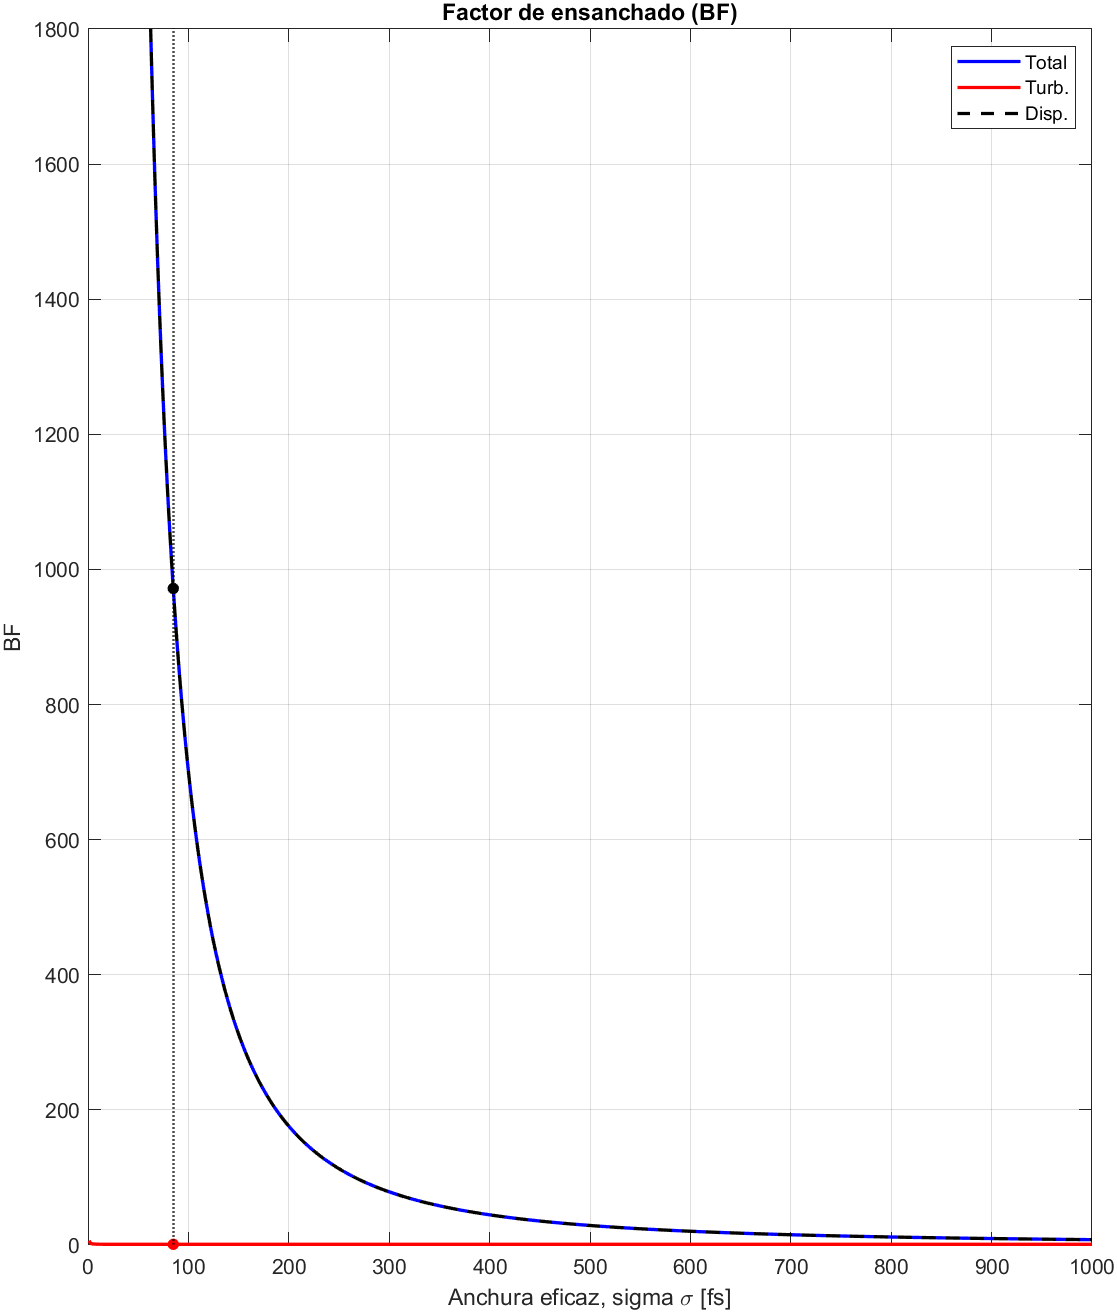
\includegraphics[width=0.9\textwidth]{figuras/ocn_comb_C1_Deb.png}
\caption{Barrido del factor de ensanchado en función de la anchura eficaz del pulso para un enlace oceánico, considerando dispersión cromática y turbulencia débil}
\label{fig_oceano_comb_debil}
\end{figure}

\paragraph{Régimen de turbulencia moderada}
A continuación, se considera un régimen de turbulencia oceánica moderada, caracterizado por $\epsilon=10^{-6}\,\mathrm{m^2/s^3}$ y $\chi_T=10^{-8}\,\mathrm{K^2/s}$.

\begin{table}[H]
\centering
\hspace*{-0.6cm}
\renewcommand{\arraystretch}{1.2}
\begin{tabular}{|l|c|}
\hline
\multicolumn{2}{|c|}{\textbf{Turbulencia oceánica moderada}} \\
\hline
Factor de ensanchamiento por dispersión, $BF_{\mathrm{disp}}$ & 971.80 \\
Factor de ensanchamiento por turbulencia, $BF_{\mathrm{turb}}$ & 1.06 \\
Factor de ensanchamiento total, $BF_{\mathrm{total}}$ & 971.80 \\
\hline
Duración final por dispersión [ps] & 194.30 \\
Duración final por turbulencia [ps] & 0.21 \\
Duración final total [ps] & 194.30 \\
\hline
\end{tabular}
\caption{Resultados del efecto combinado de dispersión cromática y turbulencia moderada en un enlace oceánico}
\label{tabla_oceano_comb_moderada}
\end{table}


En este caso, la turbulencia introduce un ensanchamiento ligeramente mayor que en el régimen débil, pero su contribución sigue siendo despreciable frente al efecto dispersivo.



\begin{figure}[H]
\centering
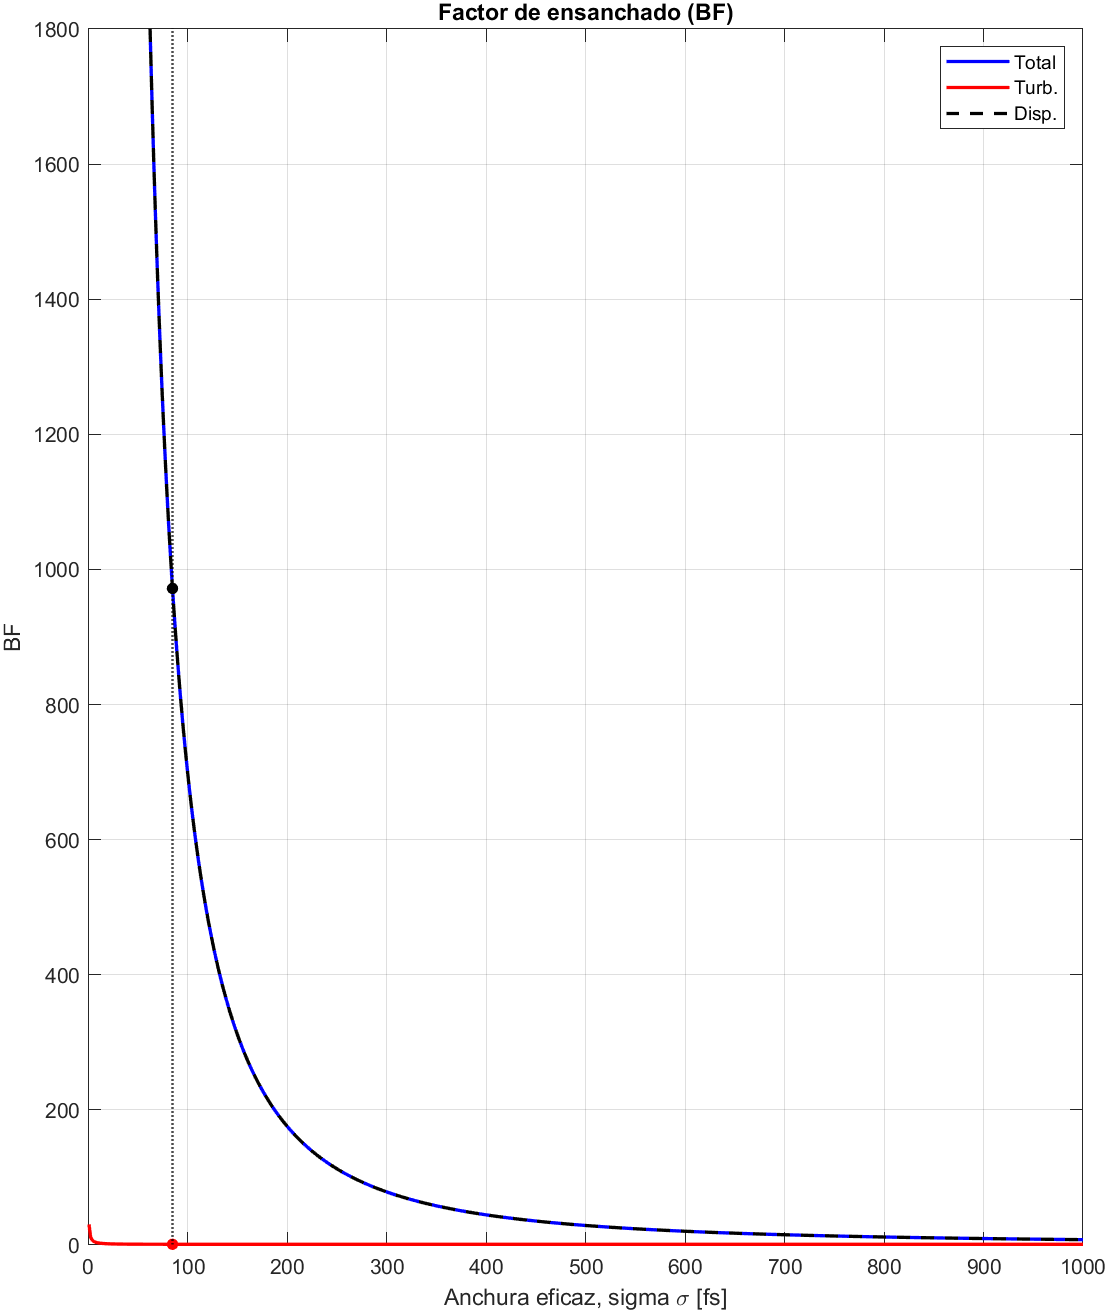
\includegraphics[width=0.9\textwidth]{figuras/ocn_comb_C1_Mod.png}
\caption{Barrido del factor de ensanchado en función de la anchura eficaz del pulso para un enlace oceánico, considerando dispersión cromática y turbulencia moderada}
\label{fig_oceano_comb_moderada}
\end{figure}

\paragraph{Régimen de turbulencia fuerte}
Finalmente, se analiza el régimen de turbulencia oceánica fuerte, correspondiente a $\epsilon=10^{-4}\,\mathrm{m^2/s^3}$ y $\chi_T=10^{-6}\,\mathrm{K^2/s}$.

\begin{table}[H]
\centering
\hspace*{-0.6cm}
\renewcommand{\arraystretch}{1.2}
\begin{tabular}{|l|c|}
\hline
\multicolumn{2}{|c|}{\textbf{Turbulencia oceánica fuerte}} \\
\hline
Factor de ensanchamiento por dispersión, $BF_{\mathrm{disp}}$ & 971.83 \\
Factor de ensanchamiento por turbulencia, $BF_{\mathrm{turb}}$ & 2.24 \\
Factor de ensanchamiento total, $BF_{\mathrm{total}}$ & 971.83 \\
\hline
Duración final por dispersión [ps] & 194.36 \\
Duración final por turbulencia [ps] & 0.44 \\
Duración final total [ps] & 194.36 \\
\hline
\end{tabular}
\caption{Resultados del efecto combinado de dispersión cromática y turbulencia fuerte en un enlace oceánico}
\label{tabla_oceano_comb_fuerte}
\end{table}

\begin{figure}[H]
\centering
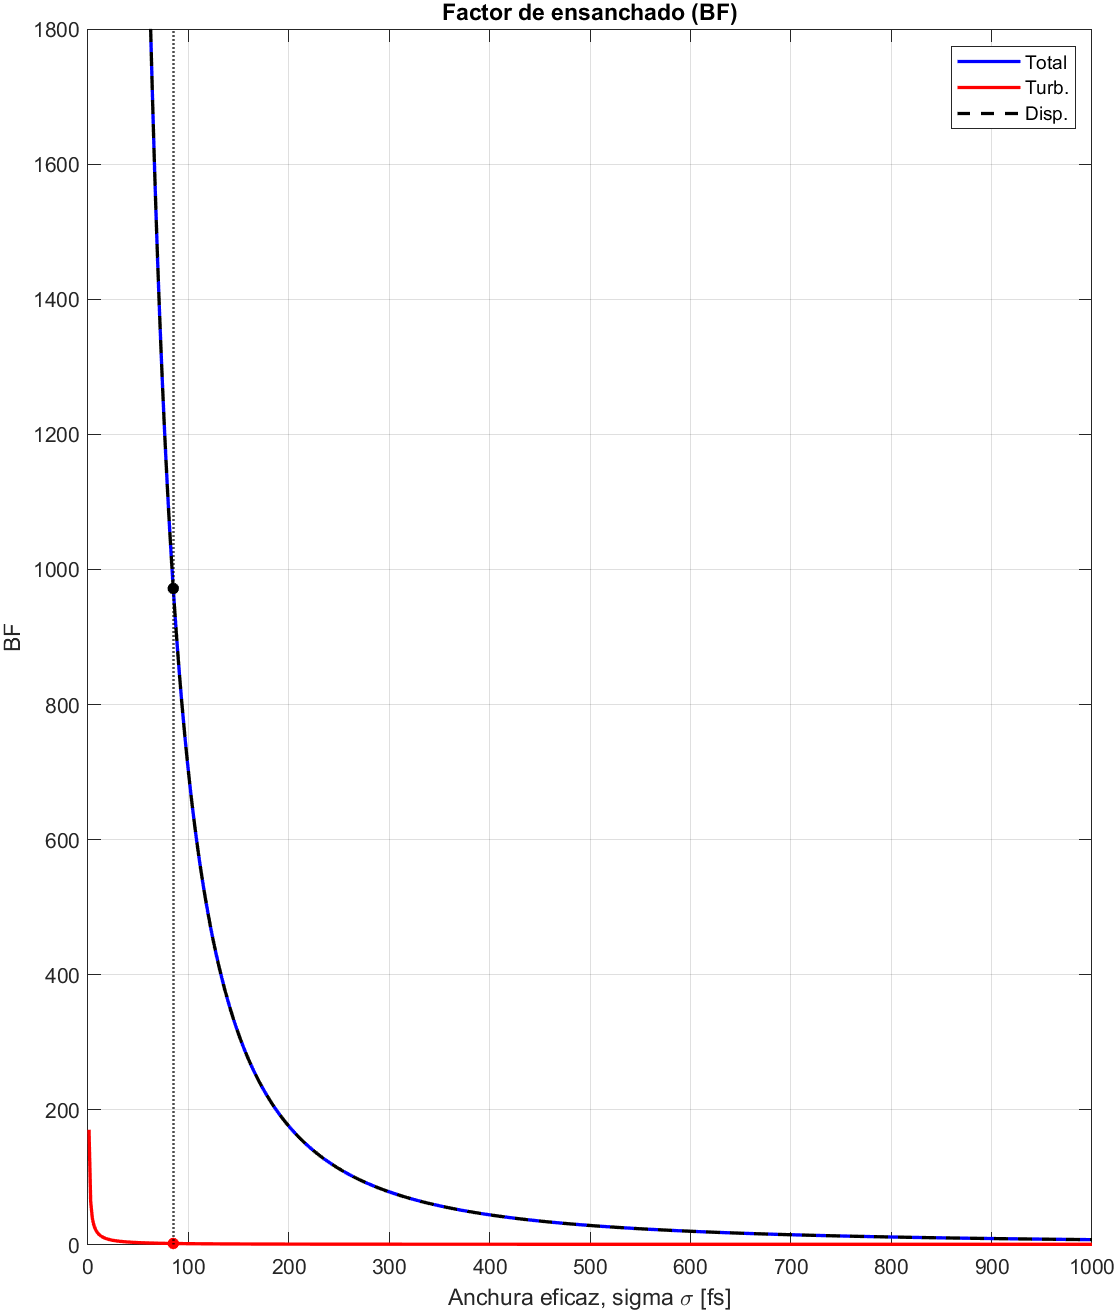
\includegraphics[width=0.9\textwidth]{figuras/ocn_comb_C1.png}
\caption{Barrido del factor de ensanchado en función de la anchura eficaz del pulso para un enlace oceánico, considerando dispersión cromática y turbulencia fuerte}
\label{fig_oceano_comb_fuerte}
\end{figure}

En este régimen, la turbulencia introduce el mayor ensanchamiento temporal observado. No obstante, incluso en estas condiciones extremas, el factor de ensanchamiento debido a la dispersión cromática es varios órdenes de magnitud superior, por lo que el comportamiento temporal del pulso sigue estando dominado por la dispersión.


\subsubsection*{Caso 2: signo en el producto $\beta_{2}C$}

En este caso se analiza la influencia de nuevo del signo del producto $\beta_{2}C$. 
Los resultados obtenidos muestran que el comportamiento del pulso en recepción es prácticamente idéntico al observado para signo positivo. Esto se explica por la extrema dominancia de la dispersión cromática en el medio oceánico. Los elevados valores del coeficiente de dispersión de segundo orden, junto con las longitudes de dispersión extremadamente cortas, provocan que el ensanchamiento temporal esté completamente gobernado por la dispersión cromática desde distancias muy reducidas. En este régimen, cualquier efecto posible compensador o reforzador queda totalmente enmascarado.


\subsubsection*{Caso 3: estudio del efecto de la longitud del enlace}
En este caso se analiza la evolución del ensanchamiento temporal al variar la distancia de propagación. Se consideran distancias de enlace \SI{10}{\meter}, \SI{25}{\meter}, \SI{50}{\meter}, \SI{75}{\meter} y \SI{100}{\meter}. Para aislar el impacto de la turbulencia en condiciones extremas, se consideran únicamente dos regímenes: turbulencia débil y turbulencia fuerte.

\paragraph{Régimen de turbulencia débil}
Los resultados obtenidos se recogen en la Tabla~\ref{tabla_oceano_longitud_debil}. Se observa que el factor de ensanchamiento asociado a la turbulencia permanece prácticamente unitario de modo que el ensanchamiento total coincide con el puramente dispersivo.


\begin{table}[H]
\centering
\hspace*{-0.8cm}
\renewcommand{\arraystretch}{1.2}
\begin{tabular}{|c|c|c|c|c|}
\hline
\textbf{Distancia [m]} &
\textbf{$BF_{\mathrm{disp}}$} &
\textbf{$BF_{\mathrm{turb}}$} &
\textbf{$BF_{\mathrm{total}}$} &
\textbf{FWHM$_{\mathrm{total}}$ [ps]} \\
\hline
10  & 97.98  & 1.0003  & 97.98  & 19.5979 \\
25  & 243.63 & 1.0007  & 243.63 & 48.72 \\
50  & 486.36 & 1.0013  & 486.36 & 97.27 \\
75  & 729.09 & 1.0020  & 729.09 & 145.82 \\
100 & 971.83 & 1.0026  & 971.83 & 194.36 \\
\hline
\end{tabular}
\caption{ Evolución del ensanchamiento temporal del pulso en función de la longitud del enlace en régimen de turbulencia débil}
\label{tabla_oceano_longitud_debil}
\end{table}


\paragraph{Régimen de turbulencia fuerte}

Los resultados obtenidos para este caso se muestran en la Tabla~\ref{tabla_oceano_longitud_fuerte}. En este régimen, la turbulencia introduce un ensanchamiento adicional. No obstante, en estas condiciones el factor de ensanchamiento total sigue estando claramente dominado por la dispersión cromática en todo el rango analizado.

\begin{table}[H]
\centering
\hspace*{-0.8cm}
\renewcommand{\arraystretch}{1.2}
\begin{tabular}{|c|c|c|c|c|}
\hline
\textbf{Distancia [m]} &
\textbf{$BF_{\mathrm{disp}}$} &
\textbf{$BF_{\mathrm{turb}}$} &
\textbf{$BF_{\mathrm{total}}$} &
\textbf{FWHM$_{\mathrm{total}}$ [ps]} \\
\hline
10  & 97.98  & 1.18  & 97.99  & 19.59 \\
25  & 243.63 & 1.41  & 243.63 & 48.72 \\
50  & 486.36 & 1.73 & 486.36 & 97.27 \\
75  & 729.09 & 2.00  & 729.10 & 145.82 \\
100 & 971.83 & 2.24  & 971.83 & 194.36 \\
\hline
\end{tabular}
\caption{ Evolución del ensanchamiento temporal del pulso en función de la longitud del enlace en régimen de turbulencia fuerte}
\label{tabla_oceano_longitud_fuerte}
\end{table}

\subsubsection*{Caso 4: cambios en la duración del pulso}

En este caso se analiza la influencia de la duración inicial del pulso gaussiano en el ensanchamiento. Se consideran cuatro duraciones iniciales: \SI{0.05}{\pico\second}, \SI{0.1}{\pico\second}, \SI{0.5}{\pico\second} y \SI{1}{\pico\second}. Para aislar el impacto de la turbulencia en condiciones extremas, se consideran únicamente dos regímenes: turbulencia débil y turbulencia fuerte.

\paragraph{Régimen de turbulencia débil}

Los resultados obtenidos para este régimen se encuentran en la Tabla~\ref{tabla_oceano_duracion_debil}.

\begin{table}[H]
\centering
\hspace*{-0.6cm}
\renewcommand{\arraystretch}{1.2}
\begin{tabular}{|c|c|c|c|c|}
\hline
\textbf{FWHM inicial [ps]} &
\textbf{$BF_{\mathrm{disp}}$} &
\textbf{$BF_{\mathrm{turb}}$} &
\textbf{$BF_{\mathrm{total}}$} &
\textbf{FWHM$_{\mathrm{total}}$ [ps]} \\
\hline
0.05 & 15564.40 & 1.0413 & 15564.40 & 778.2 \\
0.10 & 3885.97 & 1.0105 & 3885.97 & 388.5 \\
0.50 & 156.21 & 1.0004 & 156.21 & 78.10 \\
1.00 & 39.72 & 1.0001 & 39.72 & 39.72 \\
\hline
\end{tabular}
\caption{Influencia de la duración inicial del pulso en el ensanchamiento temporal tras la propagación en régimen de turbulencia débil}
\label{tabla_oceano_duracion_debil}
\end{table}
 
Se observa que el factor turbulento permanece prácticamente unitario, por lo que como ha ocurrido en otros casos anteriores, vuelve a ser la dispersión cromática el efecto dominante.

\paragraph{Régimen de turbulencia fuerte}

A continuación, se estudia el régimen de turbulencia fuerte cuyos resultados se recogen en la Tabla~\ref{tabla_oceano_duracion_fuerte}.

\begin{table}[H]
\centering
\hspace*{-0.6cm}
\renewcommand{\arraystretch}{1.2}
\begin{tabular}{|c|c|c|c|c|}
\hline
\textbf{FWHM inicial [ps]} &
\textbf{$BF_{\mathrm{disp}}$} &
\textbf{$BF_{\mathrm{turb}}$} &
\textbf{$BF_{\mathrm{total}}$} &
\textbf{FWHM$_{\mathrm{total}}$ [ps]} \\
\hline
0.05 & 15564.40 & 8.10 & 15564.40 & 778.22 \\
0.10 & 3885.97 & 4.14 & 3885.98 & 388.59 \\
0.50 & 156.21 & 1.28 & 156.21 & 78.15 \\
1.00 & 39.72 & 1.07 & 39.72 & 39.72 \\
\hline
\end{tabular}
\caption{Influencia de la duración inicial del pulso en el ensanchamiento temporal tras la propagación en régimen de turbulencia fuerte}
\label{tabla_oceano_duracion_fuerte}
\end{table}


En este régimen, la turbulencia introduce un ensanchamiento adicional más apreciable, especialmente para pulsos cortos. Sin embargo, el efecto global sigue estando completamente dominado por la dispersión cromática por varios órdenes de magnitud mayor.
